\section{CMOS-Logik}
	\begin{multicols}{2}
		\subsection{\"Ubersicht Logikfamilien}
			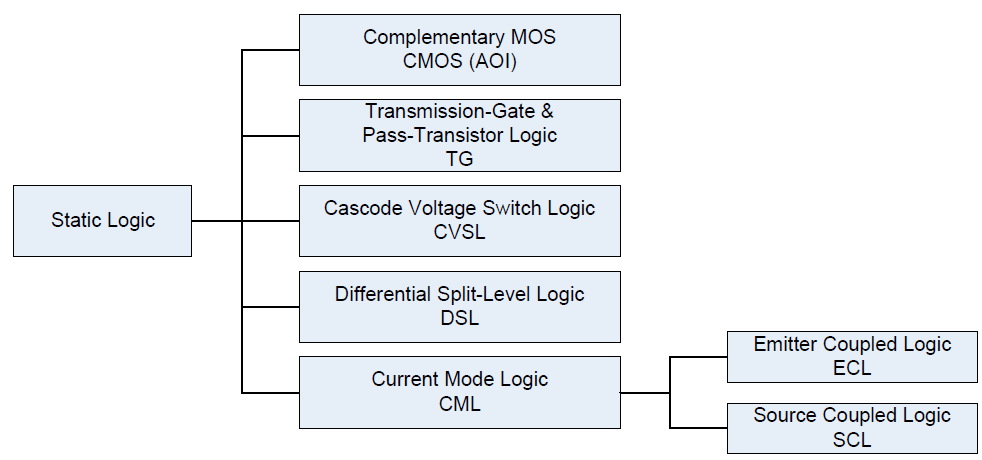
\includegraphics[width=9cm]{bilder/cmosOverview.png}
		\subsection{Staisches CMOS Modell}
			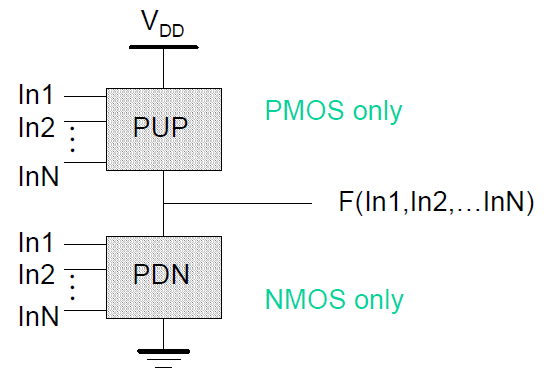
\includegraphics[width=6cm]{bilder/cmosPrinzip.png}\\
			PUN und PDN sind duale logische Netzwerke\\
	\end{multicols}
	\subsection{CMOS Inverter}
		\begin{center}
			\begin{multicols}{2}
				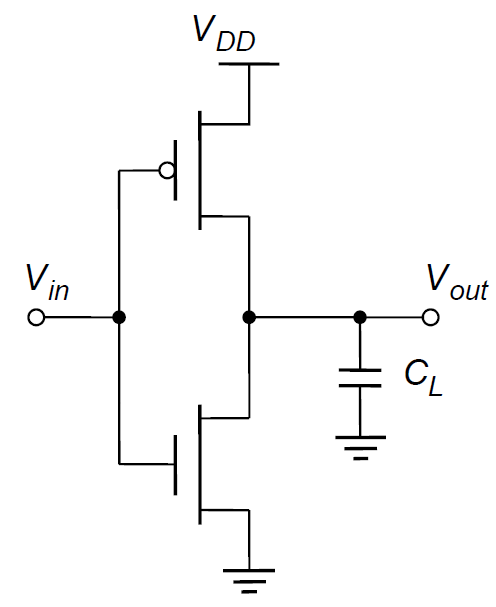
\includegraphics[width=4cm]{bilder/cmosInverterSchema.png}\\
				\columnbreak
				
				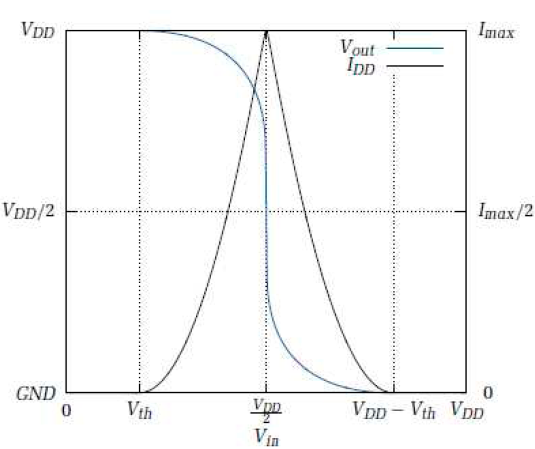
\includegraphics[width=6cm]{bilder/cmosInverterSignal.png}\\
			\end{multicols}
		\end{center}
	\subsection{Dynamische Gatter}
		\begin{multicols}{3}
			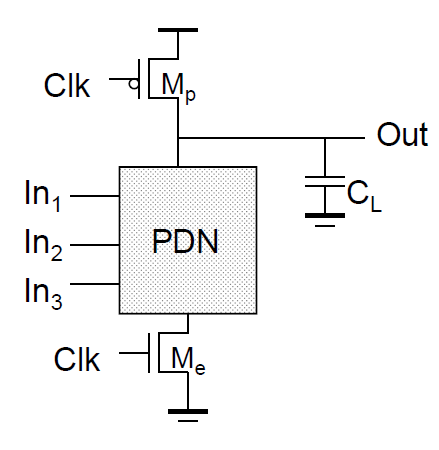
\includegraphics[width=6cm]{bilder/cmosDynPrinzip.png}\\
			\columnbreak
			
			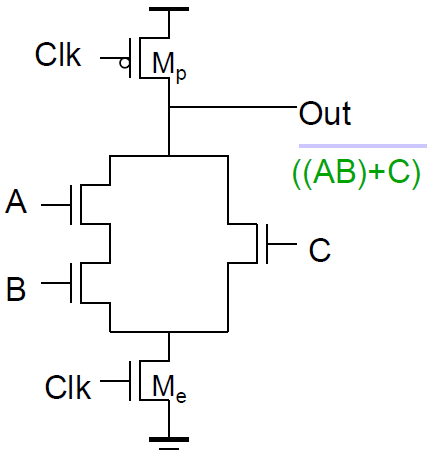
\includegraphics[width=6cm]{bilder/cmosDynSchema.png}\\
			\columnbreak
			
			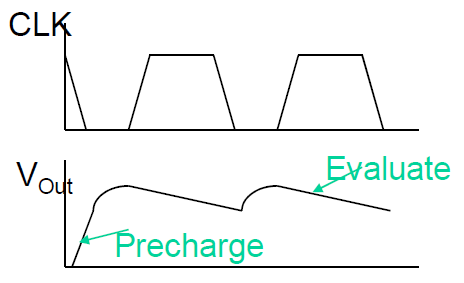
\includegraphics[width=6cm]{bilder/cmosDynSignal.png}
			\columnbreak
			
		\end{multicols}	
	